\documentclass[11pt]{article}
\usepackage[margin=0.6in]{geometry}
\usepackage[utf8]{inputenc}
\usepackage{authblk}
\usepackage{doi}
\usepackage{tcolorbox}
\usepackage{enumitem}
\usepackage{graphicx,pdflscape,multirow}
\usepackage{array}
\usepackage{xcolor}
\usepackage{multicol}
\usepackage{wrapfig,lipsum,booktabs}
\usepackage{fancybox}
\usepackage{amsmath}

\newcommand{\fixme}[1]{{\color{red} (#1)}}
\newcommand{\coloc}{\texttt{spCOCOON}}

% \renewcommand\Authfont{\fontsize{8}{14.4}\selectfont} % change author fontsize
% \renewcommand\Affilfont{\fontsize{6}{10.8}\itshape}   % change auth affil fontsize
\makeatletter % make affiliations on one line
\renewcommand\AB@affilsepx{, \protect\Affilfont}
\makeatother

\usepackage[sort&compress,square,numbers]{natbib}
\bibliographystyle{unsrtnat}

%\setmainfont{Helvetica}
\title{\coloc: Spatial Visualization Using Color Contrast Optical Illusion}
\author[1]{Boyi Guo\thanks{Corresponding author}}
\author[1]{Stephanie C. Hicks}
\affil[1]{Department of Biostatistics, Johns Hopkins Bloomberg School of Public Health, MD, USA}
\date{\today}

\begin{document}
\maketitle

\vspace{-.6in}

%% ABSTRACT ============================================================================================
\section*{Abstract}
\subsection*{Summary}
Colocalization is highly interested research questions in the analysis of spatial omics data. While many sophisticated computational models are proposed to infer the colocalization relationship between genes or proteins in the spatial context, there completely lack of intuitive spatial visualization, making interpretation extremely challenging. The biggest challenge for colocalization visualization is two sources of orthogonal information, spot colocalization and spot membership (such as spatial domain) the same spatial plot. To address this issue, we developed \coloc to display the colocalization while maintaining an intuitive representation of the surrounding spatial domain. \coloc leverages color contrast optical illusion to display spatial domains to create shadows representing different spatial domain while using different spots to denote colocalization status.  

\subsection*{Availability and implementation}
\coloc R package is freely available at Github (\url{https://github.com/boyiguo1/VisColoc}).
% and Zenodo (\fixme{add link}).


%% INTRODUCTION ============================================================================================
\section*{Introduction}
Data visualization plays a critical role in bioinformatics, serving many purposes such as verifying hypothesis, scientific communication and many more. Many researchers treat data visualization as imperative part in the cognitive process to understand hypothesis and models. With the increasly complex data generated in the bioinformatics field, tranmendous of the efforts are spend on developing new computational methods to interpolate knowledge from the data, with little efforts on how to visualize these complex data. "extracting insight from such massive, complex datasets requires development of highly tailored, innovative visual analysis methods" (O'Donoghue SI, 2021). 


 The advent of spatial omics technologies brought new outlook to study molecular, enabling researchers to investigate omics in the spatial contexts. Nevertheless, visualizing spatial data are growingly challenging due to the necessity to display omics information while maintaining the spatial relationship. Previous data visualization of omics largely relies on projecting the omics space to an embedding space, such as t-SNE and UMAP, which is infeasible for spatial omics technologies. One of the most commonly used visualization strategy is to color code each spatial unit to represent a dimension information of interest, for example the level of expression or spatial domains. A gap exists (both literally and figuratively) to simultaneously visualization two dimension of information, e.g. comparing the level of colocalization between 2 spatial domains, creating interpretation challenges. There completely lack efficient and informative visualization tools to simultaneously visualize co-localization in the spatial context, preventing the interpretation and understanding of the multi-omics profiling. While interactive platforms or 3-D visualization can alleviate this problems, these alternative solutions are not publication firendly that are normally static. It is imperative to develop a static spatial visualization that allows the simultaneous display of more than 1 dimension of information. 
 
\noindent To address this problem, we propose a novel data visualization for spatial omics data that allows simulatneous display of multiple information. The new data visaulization \textbf{leverage color contrast optical illusion}\cite{zhang_2018} to create another layer of information in spatial maps. We apply \coloc to the spatial transcriptomics dataset (Fig. 1G). The results show \fixme{colocalization}.


\section*{Methods and Implementation}
The main thrust of \coloc is to integrate another dimension of information to the spatial map using color constrast optical illusion. The color contrast optical illusion is a phenomenon where the appearance of a color is influenced by the colors surrounding it. This illusion occurs due to the way our brain processes visual information and perceives color. In a spatial map, we can construct each spatial unit as a hollow points using \texttt{ggplot2::geom\_points} where the boundary of each spatial unit are color-coded to represent one dimension of the information, working for both continuous measures such as gene expression or categorical measures such as spatial domains. It is possible to add another layer of information for an additional variable using sympols or contrast colors in side of each spot. Hence, wihtin each spatial map, multiple layers of informaiton can be displayed jointly.

\coloc is  an open source package implemented in the R programming environment. The package \coloc is constructed based on \texttt{ggplot2} and can be easily integrated to any spatial visualization pipeline, for example \texttt{spaitalLIBD} and \texttt{seurat}, that adapts \texttt{ggplot2} principles and would be able to generalized to users in both bioconductor community and seurat community

\section*{Application: Visualizing Colocalization}
To demonstrate the new visualization, we apply \coloc to visaulize the collocalization of two genes, (FYN) and (EFNA5) in the human brain dorsolateral prefrontal cortex. The two genes are previously identified that relates to SCZ expression via cell-cell communication analysis. The purpose of the visualization is to see if the density of colocalization are different across different cortex layers. Using \coloc, we can simultaneously display the colocalization and cortex layer in the same spatial plot, instead of having two saprate plots, one for cortex layer and one for colocalization, making the verification of the visual within the spaital context more straightforward and easier. 

To create a colocalization plots, \coloc follows a similar principle as \texttt{ggplot2}'s layering strategy. In the first step, we will use the funciton \texttt{spCOCOON} to create a base plot that converts a spatial transcroptimcs data structure to a plot object. In a second step, we use the function \texttt{add\_fill} to color code each spots with colcalization status, which includes three levels, spots that expressed both genes and spots that expressed either of the genes. Then, we will apply the function \texttt{add\_COCOON} to show the spatial domain (cortex layer) information. Optionally, one can apply the funciton \texttt{add\_symbol} to display another layer of information. Here, we use  the symbol to highlight the colocalization spots, i.e. the spots that expresses both genes. Because we followed the layering strategy that \texttt{ggplot2}. One can seamsely to integrate \coloc to any \texttt{ggplot2}-based spatial visiulization by piping a \texttt{ggplot2} object to \texttt{add\_COCOON} and \texttt{add\_symbol} and customize the plots using the \texttt{ggplot2} syntex and themes, greatly reduce the techinical burden to customize these new spatial plot designs.  


\section*{Summary}

While \coloc is to design to display colocalization in their spatial context, the underlying principle can be broadly applied to address visualizaiton challenges in informaiton rich visualizations. The contrast color optical illusion provides allows to add another dimension of information in any spatial visualization, which can be further used to display multi-omics presence, greatly improve the interpretability. 


%% EPILOGUE ================================================================
\section*{Acknowledgements}
B.G. would like to acknowledge Dr. Leonardo Collado Torres,  and Louise Huuki-Myers for their helpful feedback.

\vspace{0.2in}
\noindent \textit{Conflict of Interest:} none declared.

\section*{Data availability}
The spatial transcriptomics dataset was obtained from \texttt{spatialLIBD}(\url{http://research.libd.org/spatialLIBD/}). The code that generates these figures are deposited at \fixme{github manuscript repo}.

\clearpage
% \vspace{-0.1in}
\begin{wrapfigure}[13]{r}{0.8\textwidth}
\vspace{-0.3in}
\begin{center}
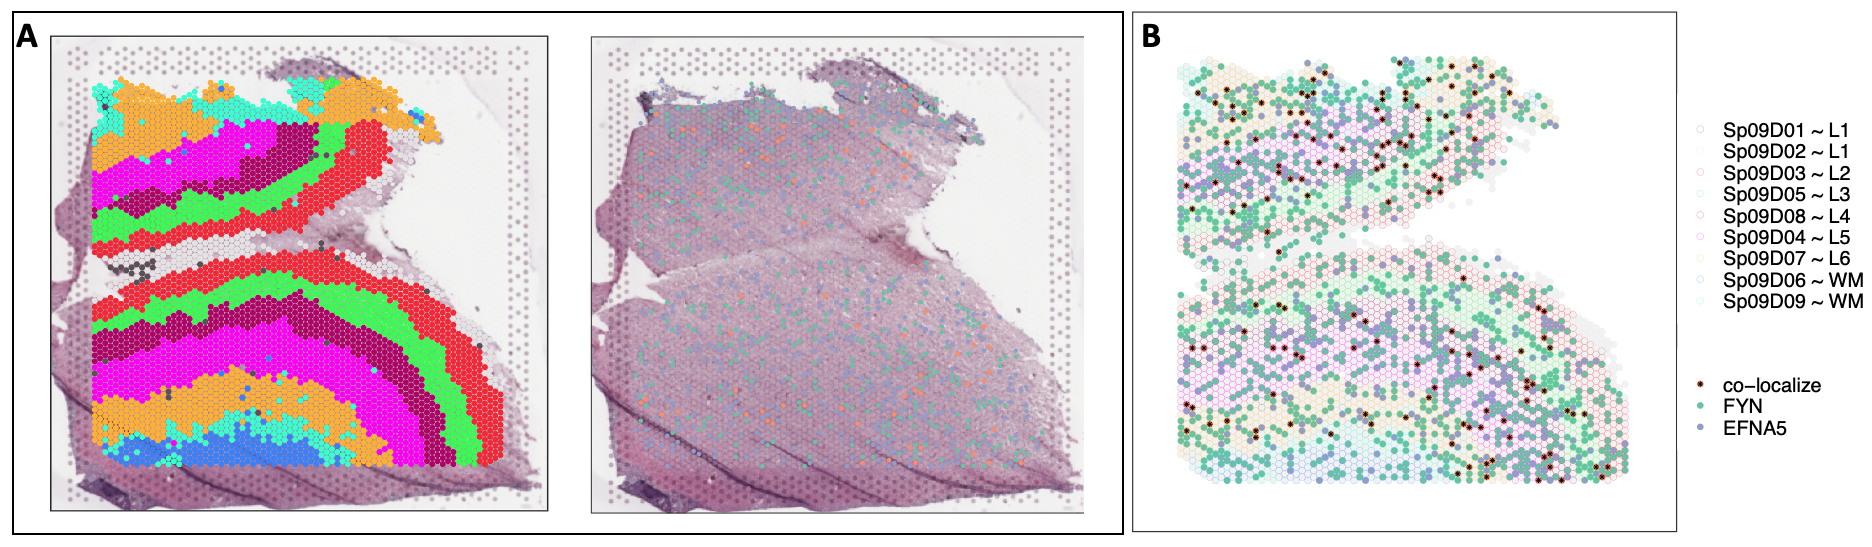
\includegraphics[width=0.78\textwidth]{figure/new_visiual.png}
\end{center}
\vspace{-0.35in}
\caption{\footnotesize \textbf{Optimized visualization interpreting co-localization in the spatial context}. (\textbf{A}) Current visualization of co-localization requires two separate plots, one to display spatial domain information and one to display co-localization, difficulty to associate the two sources of information for interpretation. (\textbf{B}) The proposed visualization is optimized to display both spatial domain and co-localization information in one plot.}
\label{fig:visual} 
\end{wrapfigure}

%% BIBLIOGRAPHY ==========================================================

\clearpage 
% \printbibliography
\bibliography{refs}

\end{document}


